% Created 2020-10-17 Sat 22:15
% Intended LaTeX compiler: pdflatex
\documentclass[11pt]{article}
\usepackage[utf8]{inputenc}
\usepackage[T1]{fontenc}
\usepackage{graphicx}
\usepackage{grffile}
\usepackage{longtable}
\usepackage{wrapfig}
\usepackage{rotating}
\usepackage[normalem]{ulem}
\usepackage{amsmath}
\usepackage{textcomp}
\usepackage{amssymb}
\usepackage{capt-of}
\usepackage{hyperref}
\usepackage {indentfirst}
\usepackage [brazilian]{babel}
\usepackage {pgf-pie}
\usepackage [a4, top = 3cm, bottom = 2cm, inner = 3cm, outer = 3cm] {geometry}
\setlength {\parindent} {3em} \hypersetup{draft}
\renewenvironment{quote}{\small\list{}{\rightmargin=0cm \leftmargin=4cm}\item[]\relax}{\endlist}
\author{Alkindar Rodrigues, Anna Julia Lima}
\date{07 de Outubro de 2019}
\title{Relatório: Remoodle\\\medskip
\large Uma reimplementação de interfaces do Moodle IFSP}
\hypersetup{
 pdfauthor={Alkindar Rodrigues, Anna Julia Lima},
 pdftitle={Relatório: Remoodle},
 pdfkeywords={},
 pdfsubject={},
 pdfcreator={Emacs 27.1 (Org mode 9.3)}, 
 pdflang={English}}
\begin{document}

\maketitle

\section*{O Moodle}
\label{sec:orgfde736f}
Neste período de pandemia, quando as universidades tiveram que se
adaptar ao ensino a distância, o Moodle se tornou uma das ferramentas
usadas para tal, ganhando ainda mais importância em comparação ao que
tinha antes de março de 2020.
Esta plataforma de gestão de aprendizagem, segundo consta em seu
portal, promete auxiliar o ensino em diversas instituições provendo
``um sistema único, robusto, seguro e integrado''\footnote{Esta informação pode ser conferida na documentação da
plataforma, \href{https://docs.moodle.org/39/en/About\_Moodle\#Highly\_flexible\_and\_fully\_customisable}{disponivel aqui}, acessado em 07 de outrubro de 2020.}, mas que ao mesmo
tempo é altamente flexível, tanto em suas funcionalidades quanto em
sua interface.

Para tanto, as versões do sistema Moodle são colocadas em produção
a pedido dos próprios gestores das instituições que o utilizam, sendo
cada instância livre das demais quanto as funções e interfaces
que decide implementar.
Para além destas variações de instância a instância, diversas opções
de \emph{layout} são disponibilizadas para os usuários, e principalmente
educadores, que recebem opções \emph{drag and drop} para construir os
espaços de disciplinas, atividades, material de estudo e áreas de
entrega de tarefas.

Desta forma, tendo em vista o papel crescente das plataformas virtuais
de ensino, escolhemos para este trabalho a reelaboração de algumas
interfaces do Moodle IFSP.
As sessões que se seguem apresentarão uma análise acerca de algumas
interfaces altualmente em uso e alguns comentários de estudantes que
usam esta plataforma para manter a rotina de estudos em isolamento
social.
Posteriormente, serão apresentadas algumas propostas de refatoração
destas interfaces, tendo em vista a sua usabilidade e guiadas pelos
comentários coletados dos usuários.

\subsection*{A interface do Moodle IFSP}
\label{sec:org544adae}
No escopo deste projeto, escolhemos três interfaces do portal Moodle
IFSP para reimplementar: a página inicial, aberta após o login na
plataforma, a página de disciplina, relativa a cada um dos cursos em
que o aluno está matriculado e a página de entrega de tarefas.  Estas
três interfaces foram escolhidas pois forma um caso de uso bastante
comum: a entrega de uma atividade por um estudante. Prints com estas
interfaces estão disponíveis no \hyperref[sec:orgbcb1147]{Apêndice} deste documento.

\subsubsection*{O painel de cursos}
\label{sec:orgf872776}
A interface principal do Moodle IFSP, como vista nas fuguras
\ref{fig:org6c39f2d} e \ref{fig:orga96bba0}, está codificada nas cores da instuição (verde e branco)
e presenta 5 grandes áreas:
\begin{itemize}
\item Uma barra de navegação, no topo, com alguns menus \emph{drop-down} com
\emph{links} pra os diversos tipos de usuários, uma caixa de pesquisa,
alertas de notificações, \emph{chat}, email e outro menu \emph{drop-down} com
\emph{links} para acesso rápido às informações do usuário.
\item Uma barra lateral à esquerda, acessível por um botão na barra de
navegação, composta por botões para a página inicial, calendário
acadêmico, arquivos privados e um menu \emph{drop-down} com as
disciplinas em que o aluno está inscrito.
\item Uma área central, intitulada ``Resumo dos cursos'', com \emph{cards}
relativos a cada uma das disciplinas do aluno, seguida de outra área
(fora do \emph{print}) de cursos acessados recentemente, com os \emph{cards} semelhantes.
\item Uma barra lateral, cujo conteúdo completo não coube no \emph{print},
intitulada ``Linha do tempo'', com as entregas de tarefas, opções de
personalização desta (atrasadas, futuras, período de listagem),
seguida de:
\begin{itemize}
\item opções de acessiblidade;
\item usuários online;
\item calendário;
\item uma segunda lista chamada ``Próximos eventos'', com as avaliações
e tarefas futuras, e;
\item arquivos privados do usuário.
\end{itemize}
\item Um rodapé verde, com informações sobre os responsáveis sobre a
página e a localização do IFSP São Paulo.
\end{itemize}

Nota-se imediatamente alguns problemas com \emph{layout}: a repetição de
informações nesta tela, com a duplicação, das informações de
cursos atuais e tarefas futuras. Um botão para personalizar a página
flutua à direita, acima da barra lateral. A barra lateral à direita é
desproporcionalmente grande em relação aos demais elementos da página.

\subsubsection*{A página de disciplina}
\label{sec:org859912d}
Dentre as interfaces do portal Moodle, esta é uma das mais flexíveis
com relação ao \emph{layout}.  As figuras \ref{fig:orgef731fb}, \ref{fig:org1103064} e
\ref{fig:org64d1f32} apresentam \emph{prints} parciais de páginas de disciplinas
ofertadas no segundo semestre de 2020, enfocando a disposição das
aulas em cada uma. Consideramos estes \emph{prints} são ilustrativos acerca
da enorme flexiblidade em esta interface apresenta:

Vemos na figura \ref{fig:orgef731fb} uma árvore de tópicos. No primeiro nível
dela, cada elemento diz respeito a uma aula, com seu número e tópico
em texto grande.  Um nivel abaixo, vários \emph{links} com símbolo de
arquivos em pdf, contendo os materiais de aula.  Alguns elementos
deste nível, referentes a exercícios a serem entregues, possuem
subtópicos, com \emph{links} que levam à pagina de entrega de tarefas.  Os
tópicos no primeiro nível separados por uma linha horizontal, que
delimita o espaço de cada aula.

Um segundo \emph{layout} aplicado a esta página esta apresentado na imagem
\ref{fig:org1103064} neste, alguns \emph{links} foram disponiblizados no topo da
página, com um acesso a espaços de avisos e retirada de dúvidas, aulas
síncronas gravadas e uma calculadora online. Logo abaixo destes \emph{links},
vários blocos azuis se sobrepões, em um esquema de \emph{tabs} que expandem
o conteudo de uma aula abaixo (fora do \emph{print}). Estas podem ter um
tamanho qualquer, incluir videos, documentos pdf, word ou outros. Como
o espaço ocupado pelas \emph{tabs} é consideravelmente maior que a largura
da página, a linha é quebrada, descaracterizando uma barra de \emph{tabs}.

Por fim, o \emph{layout} apresentado na \ref{fig:org64d1f32} é semelhante ao da figura
\ref{fig:orgef731fb}: é apresentada uma lista de caixas, com um título em letras
grandes e azuis, indicando um \emph{links}. No canto direito inferior das
caixas há alguns rótulos, indicando os materiais associados à aula:
documentos, tarefas, \emph{links} externos, e indicadores de progresso,
para tarefas com mais de uma etapa.

\subsubsection*{A página de entrega de tarefas}
\label{sec:org98d8833}
A área de entrga de tarefa, como vista nas figuras \ref{fig:org1f2a93f} e
\ref{fig:org1c75e51} apresenta a mesma barra de navegação presente nas páginas
anteriores. O corpo da página é composto apenas por uma área, com um
título, instruções e uma tabela com as informações de envio. Dentre as
opções de envio, é possível enviar arquivos ou textos, além de
comentários sobre o envio que podem ser adicionados a qualquer
momento.

Após o envio, a linha da tabela ``Status de envio'' fica tingida de
verde, evidenciando que a tarefa foi cumprida. Posteiormente, quando a
avaliação for finalizada, a linha seguinte, ``Status da avaliação''
também é colorida em verde, como visto na figura \ref{fig:org908988e} e uma
segunda tabela aparece, logo abaixo da primeira, com as informações de
avaliação (nota, data de avaliação, avaliador e comentários.)

Para realizar o envio de uma tarefa, por arquivo, ao clicar no botão
(fora do print), abre-se a página vista na figura \ref{fig:orga777d26}. Esta
contém as mesmas instruções da página anterior e uma tabela com uma
linha contendo a área de \emph{upload} de arquivo, e outra com botões de
ação: salvar e cancelar. Abaixo o rodapé com setas de navegação, para
o tópico anterior. Na linha de envio de arquivos, há dois botões
também, um para criar uma pasta virtual e organizar os arquivos
enviados, outro que abre o \emph{pop-up} de seleção de arquivo.

Este \emph{pop-up}, apresentado na figura \ref{fig:org28d28de}, quando aberto,
escurece a página por baixo, desativando todos os cliques nela.  Para
além disso, ele apresenta um botão de \emph{upload} de arquivo, e um
formulário com opções de como salvar o arquivo, com o nome a ser
salvo, autor e a licensa de uso. À esquerda, estão algumas abas
disponíveis, com diferentes fontes dos arquivos: \emph{upload}, recentes,
arquivos privados e \emph{Wikimedia}.


\subsection*{Comentários de usuários sobre a inferface do Moodle IFSP}
\label{sec:orgfd8fdac}
Apresentada as interfaces do Moodle escolhidas para análise neste
projeto, podemos destacar algumas opiniões acerca desta interface,
oferecidas por alguns usários. A coleta de dados foi feita por meio de
um forms no google, disponível \href{https://forms.gle/U3KtLT2xPk4pn2q5A}{aqui}, de forma a garantir a anomidade
dos usuários. 32 alunos do Instituto Federal de São Paulo responderam:

Podemos ver, pelo gráfico \ref{fig:org8814b61} que metade das pessoas
aprenderam a usar o Moodle de forma fácil, e que 75\% dos usuários nao
tem grandes dificuldades de uso hoje.  Entretanto, comparando com o
gráfico \ref{fig:org58661d7}, das pessoas que tiveram dificuldade moderada para
aprender a usar a plataforma, algumas consideram a experiência de uso
atual como díficl, indicando que não aprenderam a usá-la de forma
satisfatória.


Apesar de os alunos conseguirem usar a plataforma, muitos ainda tem
opiniões desfavoráveis sobre o seu \emph{layout}, como mostram os gráficos
\ref{fig:org998f94a} e \ref{fig:orgab6de9a}. Por volta de 60\% não consideram o Moodle
organizado e tem dificuldades para usar o painel de cursos. Uma
resposta fala especficamente sobre isso. O aluno:

\begin{quote}
[\ldots{}] tinha muita dificuldade do uso das disciplinas, até
que comecei a usar a ferramenta de favoritar a disciplina, assim
concentrei todas as disciplinas que estou cursando atualmente num só
painel (o painel de favoritos), ficando assim de fácil acesso.
\end{quote}

Muitos outros alunos citam a enorme flexibilidade na hora de
confirgurar os \emph{layouts} na página de disciplina como um ponto
negativo:

\begin{quote}
As diferentes formas possíveis de personalizar o espaço virtual da
matéria, podendo gerar certa confusão e/ou desorganização devido as
diferenças. Um modelo único seria mais desejável
\end{quote}


\begin{quote}
Da bagunça, deveria ter um padrão, principalmente no ambiente de cada
disciplina O visual poderia ser mais limpo, tem muita informação
desnecessária
\end{quote}

Comparando com as respostas positivas, acerca do que os alunos gostam
da plataforma, percebemos que a funcionalidades implementadas são
desejadas, mas a forma como são feitas deixa a desejar e provocam os
comentários negativos acima.
Os alunos dizem:

\begin{quote}
A forma como as atividades ficam no painel para nos lembrar, é muito
  bom.\\
A forma como são entregues as atividades
\end{quote}

O calendário com as datas de entrega é uma \emph{feature} bastante
elogiada, como vemos:

\begin{quote}
Calendário para a verificação das datas das tarefas
\end{quote}

\begin{quote}
Gosto bastante de utilizar o calendário para me orientar sobre quais
são os trabalhos que tenho pendentes.
\end{quote}


\section*{Propostas de refatoração}
\label{sec:orgf9d512f}
A partir destes comentários, que apontam a necessidade de
reformular a interface do Moodle IFSP, elaboramos a seguinte lista de
critérios para a interface proposta:

\begin{itemize}
\item Para a página do painel de cursos:
\begin{itemize}
\item Simplificar do \emph{layouts} do painel de cursos,
\item Remover a duplicação dos na área de favoritados,
\item Permitir a fltragem de cursos conforme semestre, sigla, professor e
favoritos.
\vspace{1em}

\item Remover o acesso ao menu principal à esquerda.
\vspace{1em}

\item Unificar as duas listas de atividades por entregar,
\item Agrupar os demais campos da barra lateral em apenas um espaço,
cujo conteúdo é escolhido junto ao título do espaço,
\item Manter esta barra à direita com a altura da tela, no máximo,
\item Agrupar as atividades por entregar segundo as disciplinas,
\item Manter da ferramenta de filtragem  da lista de atividades.
\vspace{1em}

\item Refazer o \emph{footer} dá página, ocupando menos espaço e apresentando
as informações relevantes sobre a instituição e os responsáveis
pela plataforma.
\vspace{1em}
\end{itemize}

\item Para a página de disciplina:
\begin{itemize}
\item Unificar os \emph{layouts} disponíveis em uma estutura simplificada,
\item Apresentar o espaço com a ementa à direita,
\item Um espaço com as aulas e rótulos relevantes à esquerda, com
rolagem independente da página,
\item Destacar aulas com atividades pendentes com uma coloração sutil.
\vspace{1em}
\end{itemize}

\item Para a página de uma aula:
\begin{itemize}
\item Unificar os \emph{layouts} em uma esturutura simplificada,
\item Apresentar o título, textos e demais recusros, inseridos
diretamente no Moodle em um espaço no topo da página,
\item Abaixo, em um carrossel, os links, arquivos e tarefas
disponibilizados para a aula.
\begin{itemize}
\item Tarefas já concluídas estariam marcadas sutimelmente em verde,
atrasadas em vermelho.
\vspace{1em}
\end{itemize}
\end{itemize}

\item Para a área de entrega de tarefa.
\begin{itemize}
\item Simplificação do \emph{layout} de tabela da página, com melhor uso do
espaço negativo e coloração.
\item Incorporação do \emph{pop-up} de \emph{upload} de arquvivo à página, como um
campo da tabela.
\item Junção de ambas as tabelas (envio e \emph{feedback} do professor).
\end{itemize}
\end{itemize}

\subsection*{Wireframes}
\label{sec:orgcf61f24}
Com base nos critérios e objetivos acima expostos, e como guia no
desenvolvimento do protótipo desta interface, preparamos os seguintes
\emph{wireframes} para este projeto.



\section*{Conclusão}
\label{sec:org48f66c3}


\section*{Apêndice}
\label{sec:orgbcb1147}
\setcounter{figure}{0}
\renewcommand{\figurename}{Fig.}
\begin{figure}[htbp]
\centering
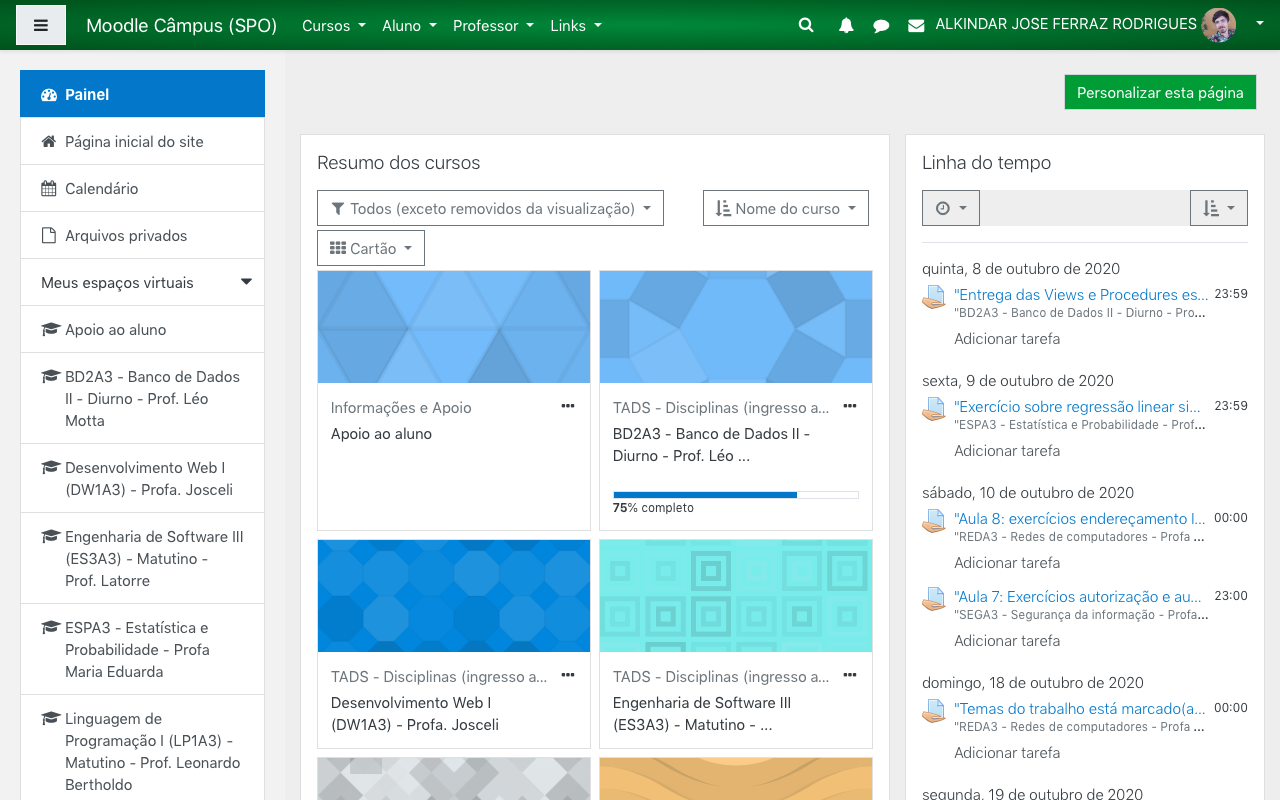
\includegraphics[width=.9\linewidth]{./media/painel.png}
\caption{\label{fig:org6c39f2d}Painel de cursos do Moodle IFSP}
\end{figure}
\begin{figure}[htbp]
\centering
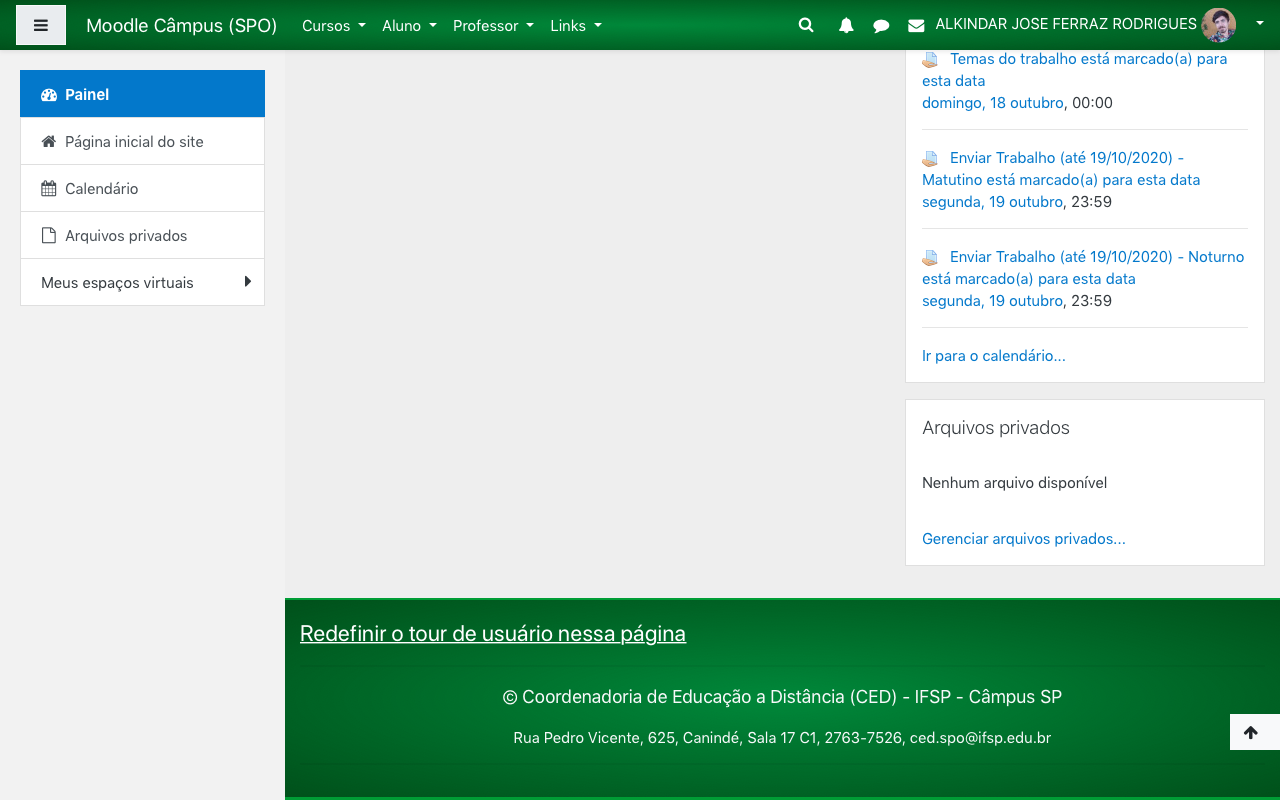
\includegraphics[width=.9\linewidth]{./media/painel_fim.png}
\caption{\label{fig:orga96bba0}Fim da página de painel de cursos do Moodle IFSP}
\end{figure}
\begin{figure}[htbp]
\centering
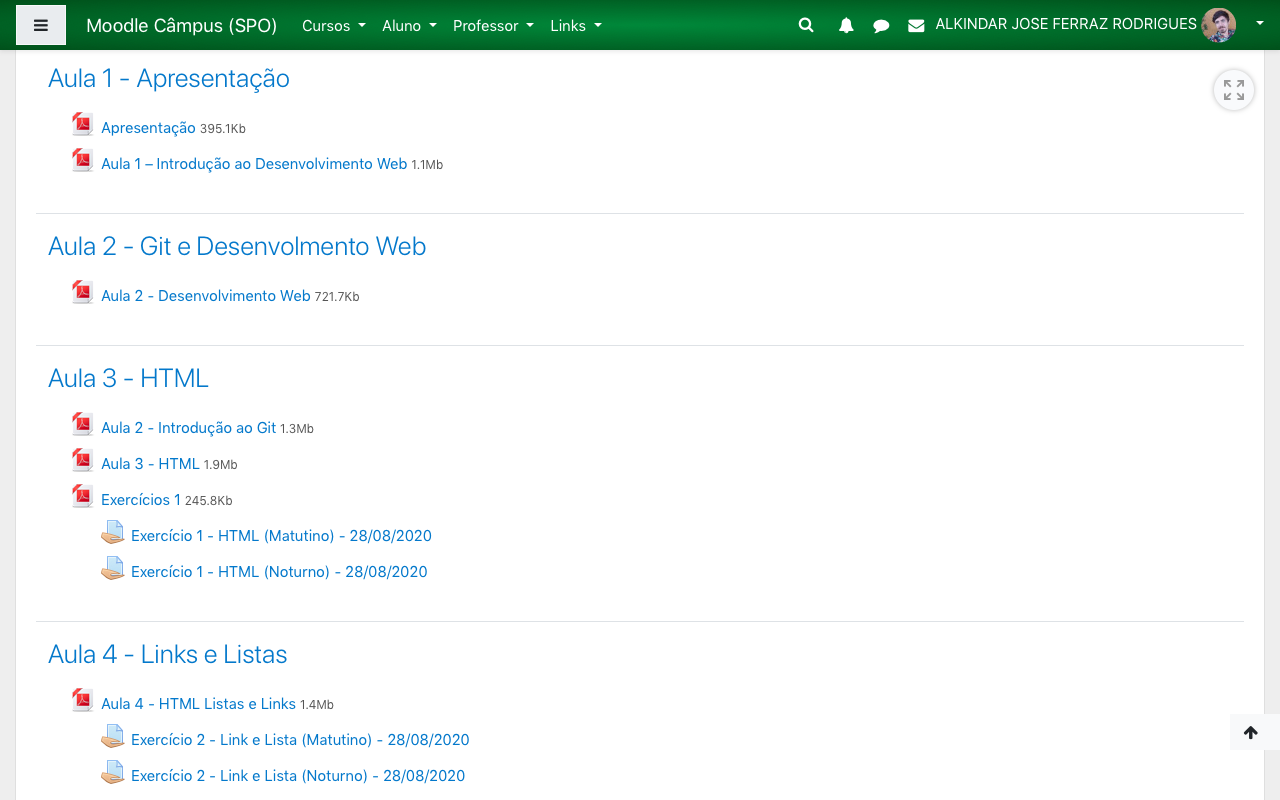
\includegraphics[width=.9\linewidth]{./media/disc_1.png}
\caption[\emph{Layout}]{\label{fig:orgef731fb}\emph{Layout} da página de disciplina: aulas e arquivos.}
\end{figure}
\begin{figure}[htbp]
\centering
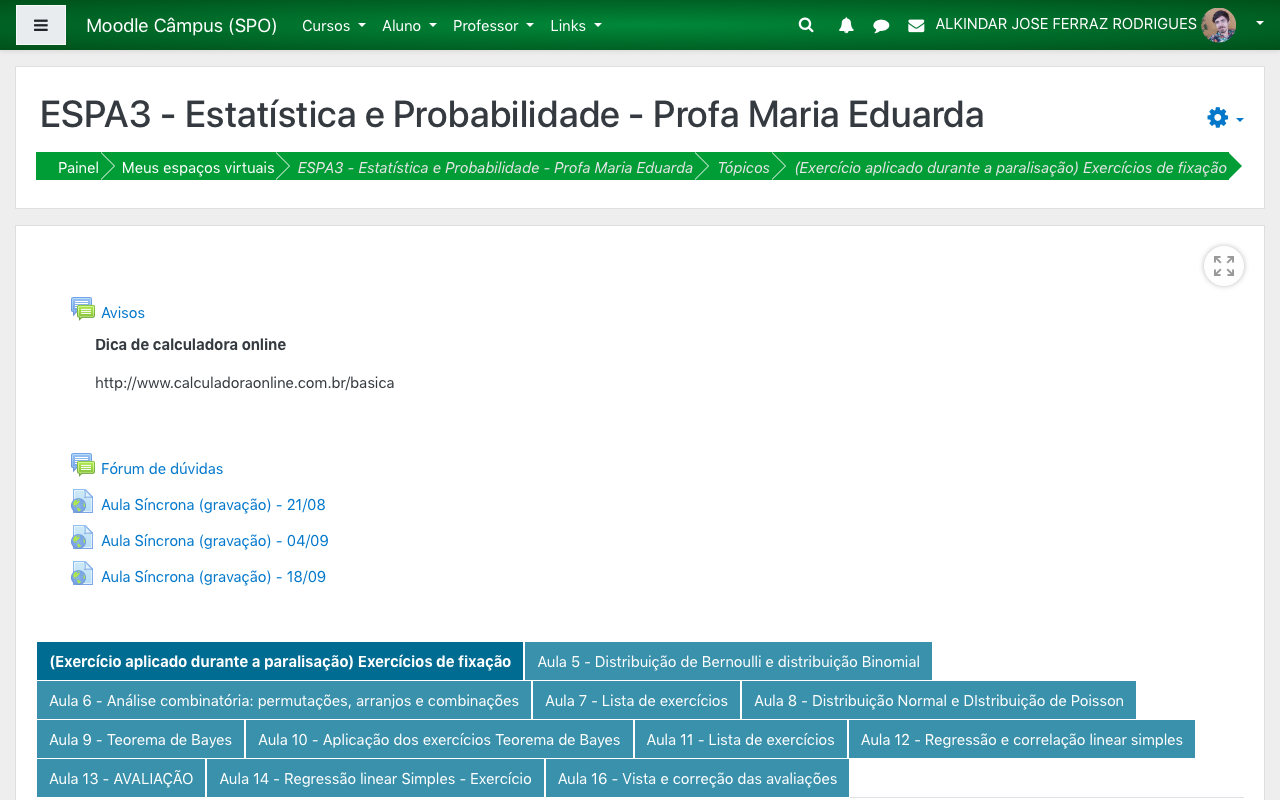
\includegraphics[width=.9\linewidth]{./media/disc_2.png}
\caption[\emph{tab}]{\label{fig:org1103064}\emph{Layout} da página de disciplina: tópicos em \emph{tab} que expandem o conteúdo da aula.}
\end{figure}
\begin{figure}[htbp]
\centering
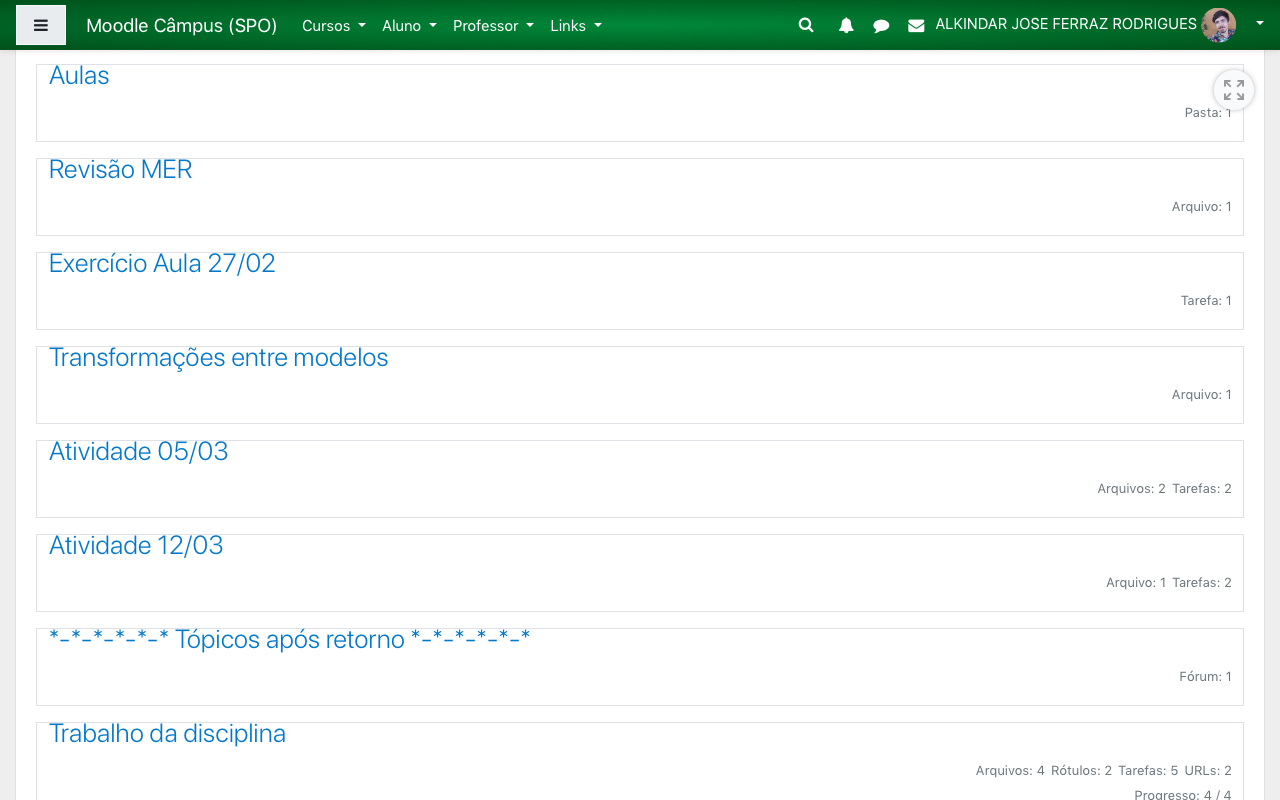
\includegraphics[width=.9\linewidth]{./media/disc_3.png}
\caption[\emph{Layout}]{\label{fig:org64d1f32}\emph{Layout} da página de disciplinas: tópicos em caixas largas, com detalhes sobre os materiais disponíveis a direita.}
\end{figure}
\begin{figure}[htbp]
\centering
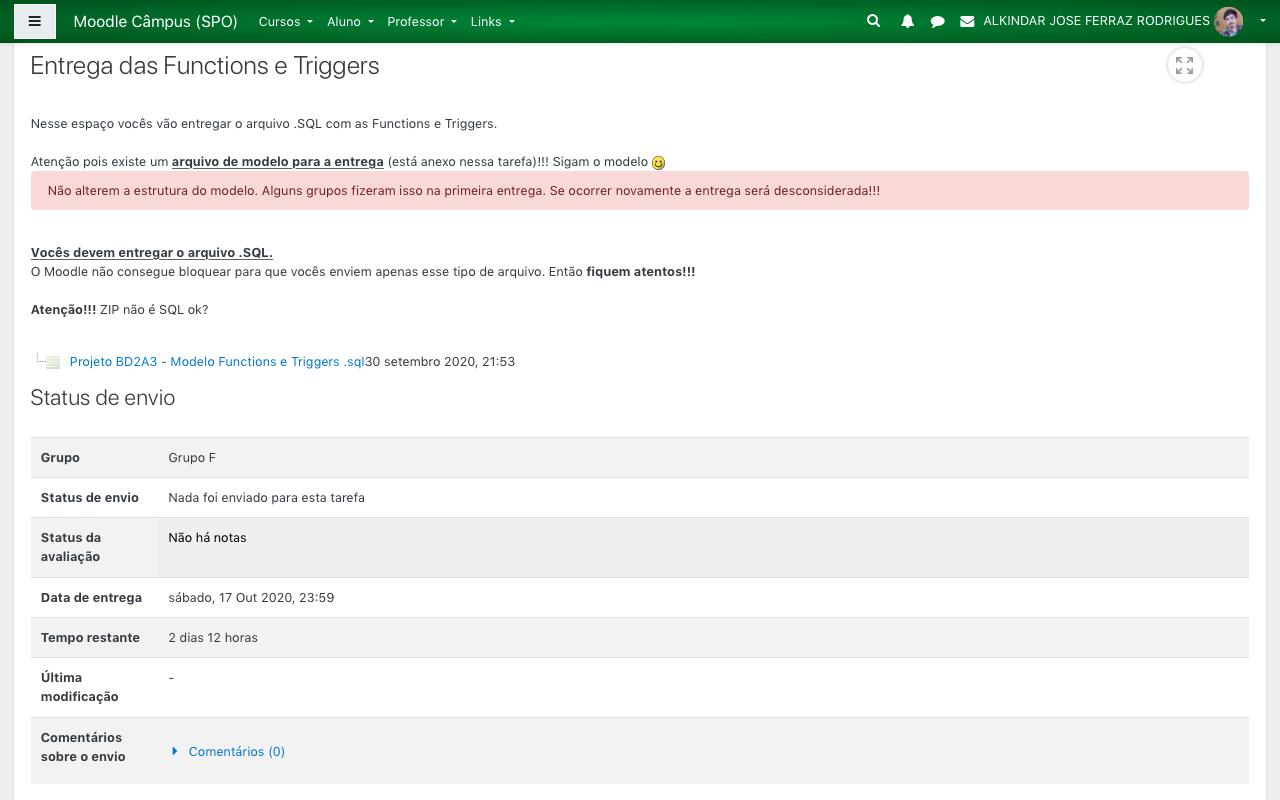
\includegraphics[width=.9\linewidth]{./media/entrega_1.png}
\caption[\emph{Layout}]{\label{fig:org1f2a93f}\emph{Layout} da página de entrega de tarefas, com a atividade ainda por enviar.}
\end{figure}
\begin{figure}[htbp]
\centering
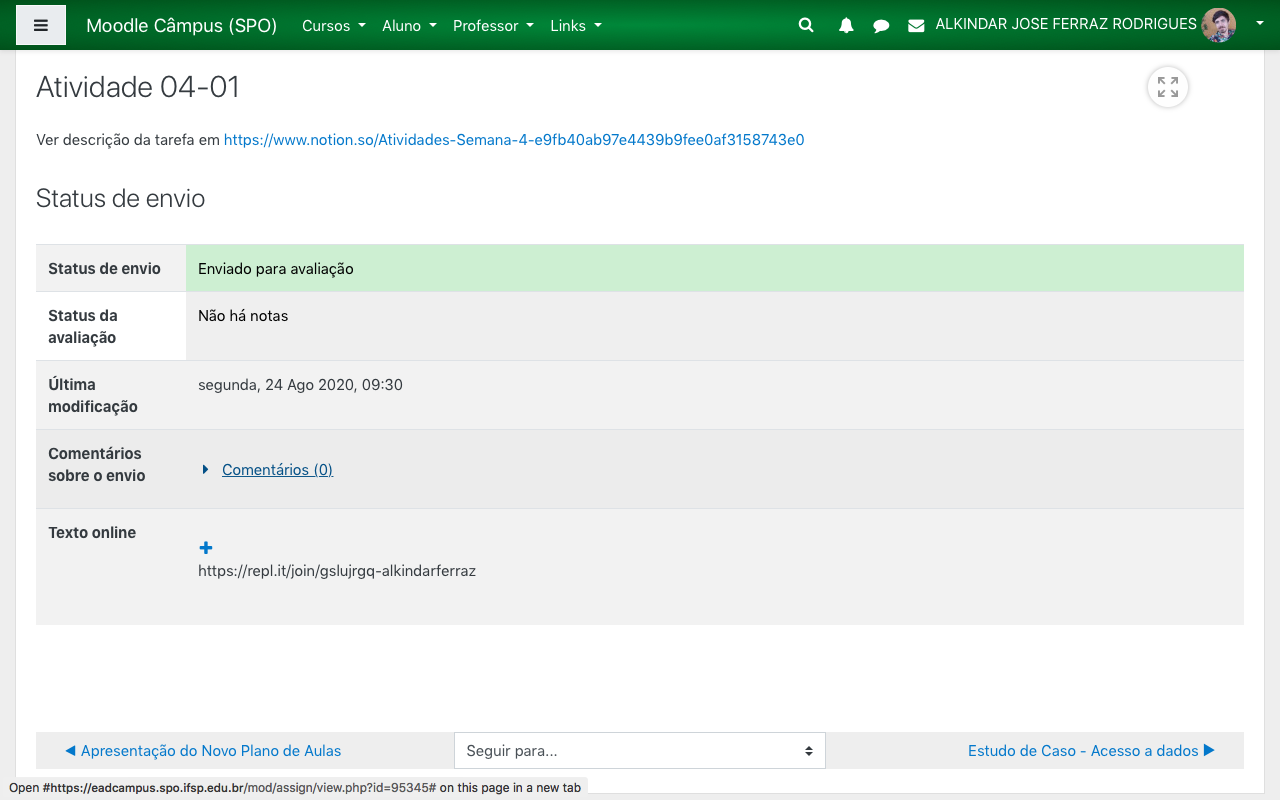
\includegraphics[width=.9\linewidth]{./media/entrega_2.png}
\caption[\emph{Layout}]{\label{fig:org1c75e51}\emph{Layout} da página de entrega de tarefas, com a atividade enviada.}
\end{figure}
\begin{figure}[htbp]
\centering
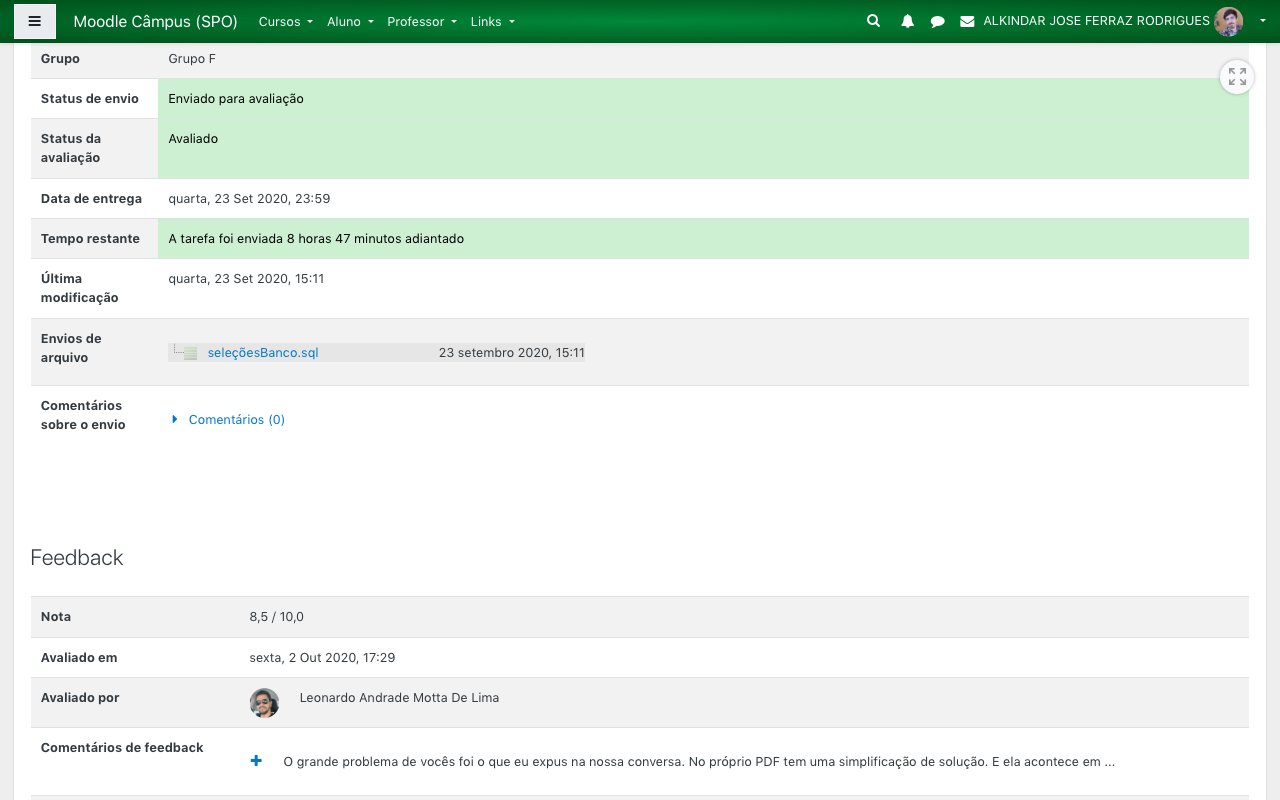
\includegraphics[width=.9\linewidth]{./media/entrega_3.png}
\caption[\emph{Layout}]{\label{fig:org908988e}\emph{Layout} da página de entrega de tarefas, com a atividade avaliada.}
\end{figure}
\begin{figure}[htbp]
\centering
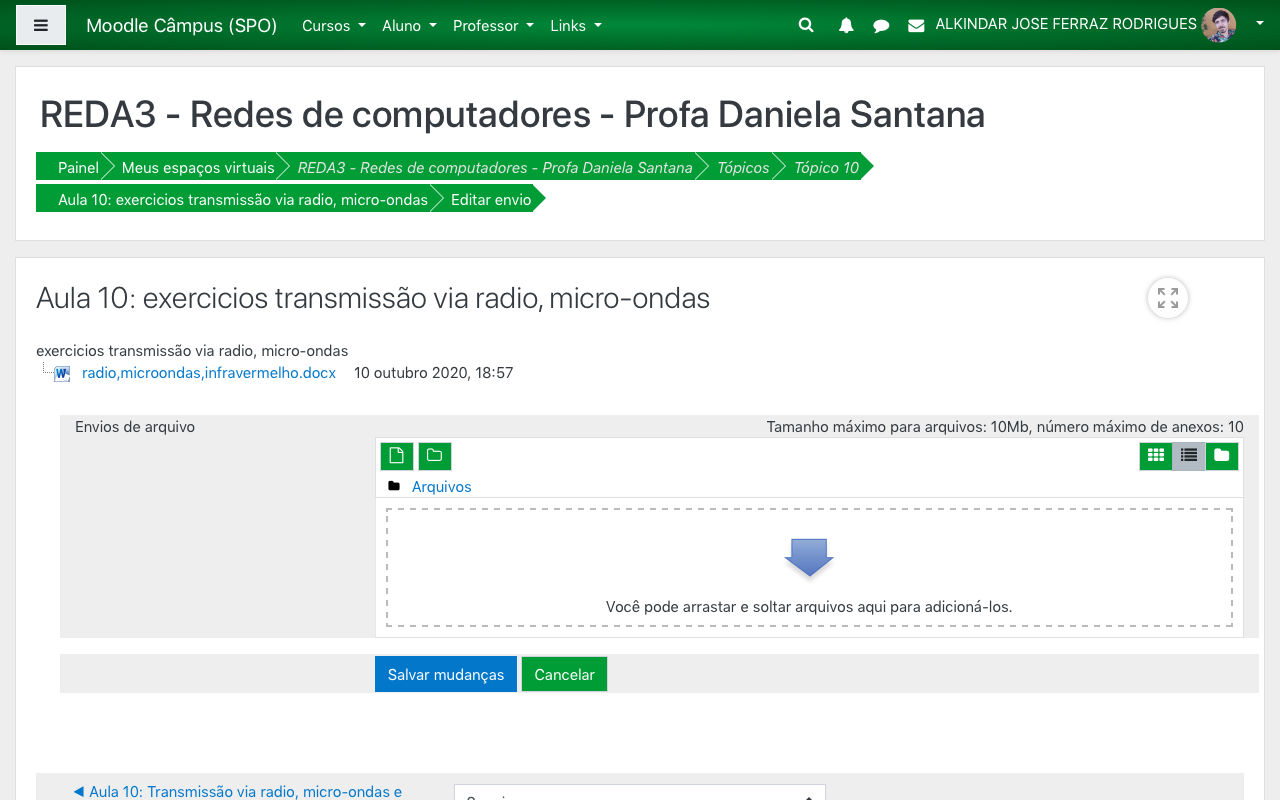
\includegraphics[width=.9\linewidth]{./media/arquivos_1.png}
\caption[\emph{Layout}]{\label{fig:orga777d26}\emph{Layout} da página de upload de arquivos.}
\end{figure}
\begin{figure}[htbp]
\centering
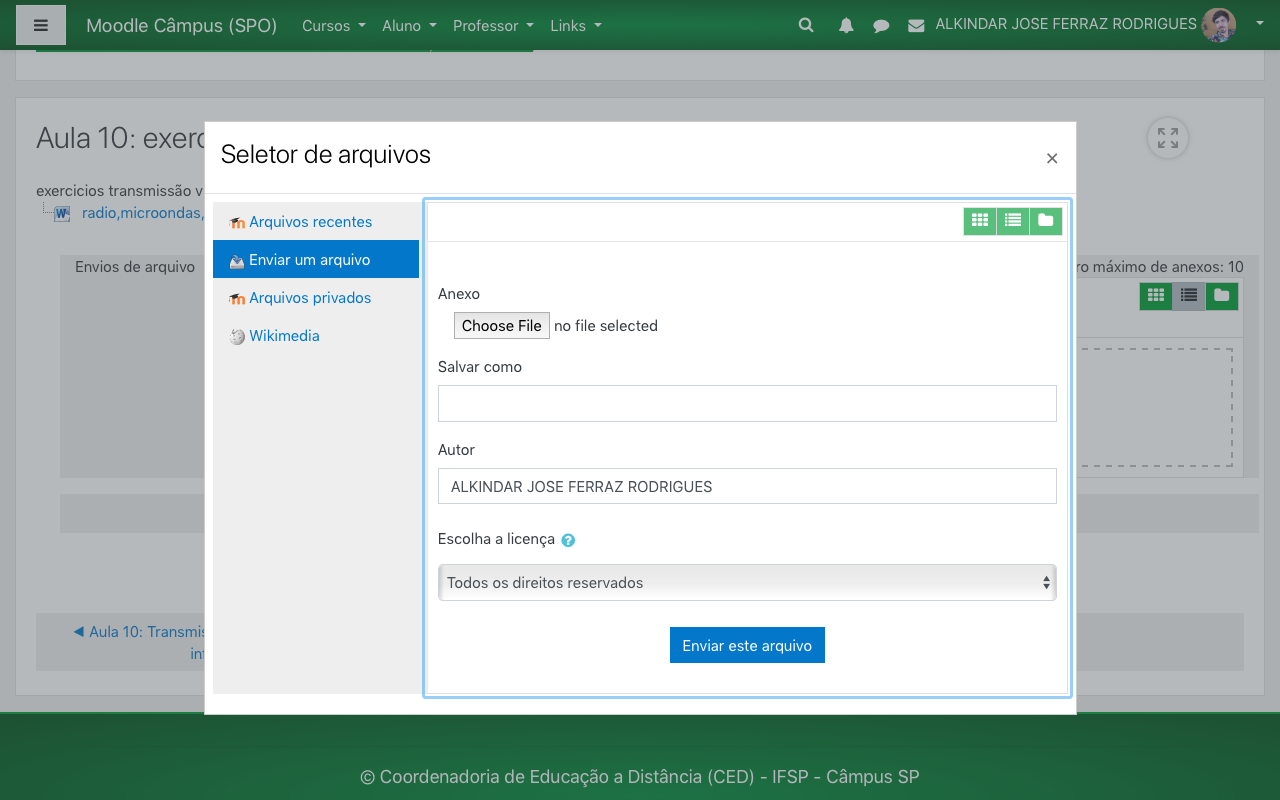
\includegraphics[width=.9\linewidth]{./media/arquivos_2.png}
\caption[\emph{pop-up}]{\label{fig:org28d28de}\emph{Layout} do \emph{pop-up} de seletor de arquivos.}
\end{figure}

\setcounter{figure}{0}
\renewcommand{\figurename}{Gráfico}
\begin{figure}[htbp]
\centering
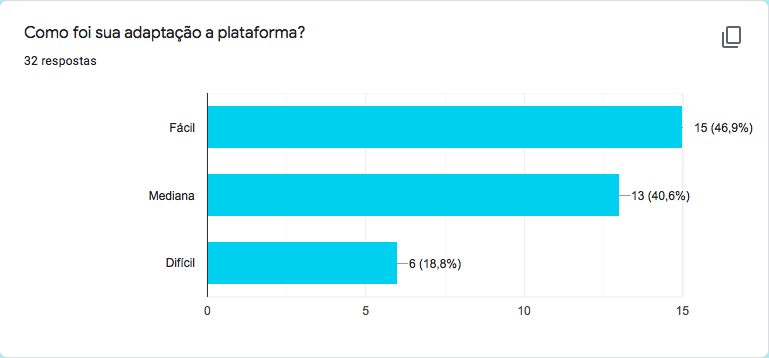
\includegraphics[width=.9\linewidth]{./media/grafico_adaptacao.png}
\caption{\label{fig:org8814b61}Porcentagem de alunos que disseram se adaptar com facilidade à plataforma.}
\end{figure}
\begin{figure}[htbp]
\centering
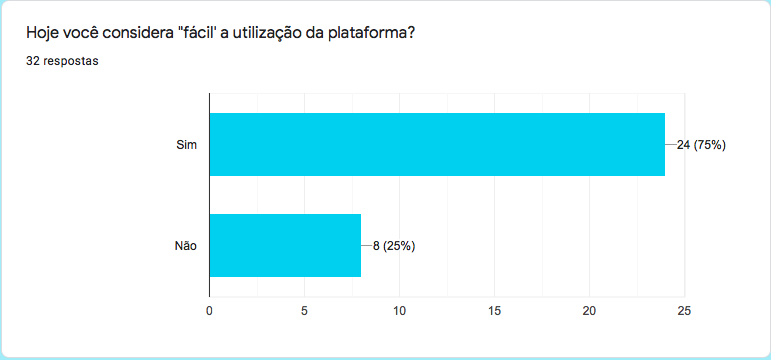
\includegraphics[width=.9\linewidth]{./media/grafico_uso.png}
\caption{\label{fig:org58661d7}Porcentagem de alunos que disseram ter facilidade de usar a plataforma.}
\end{figure}
\begin{figure}[htbp]
\centering
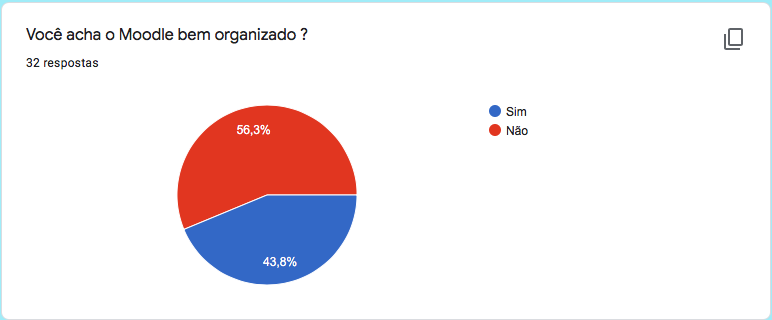
\includegraphics[width=.9\linewidth]{./media/grafico_organizacao.png}
\caption{\label{fig:org998f94a}Porcentagem de alunos que consideram a plataforma organizada.}
\end{figure}
\begin{figure}[htbp]
\centering
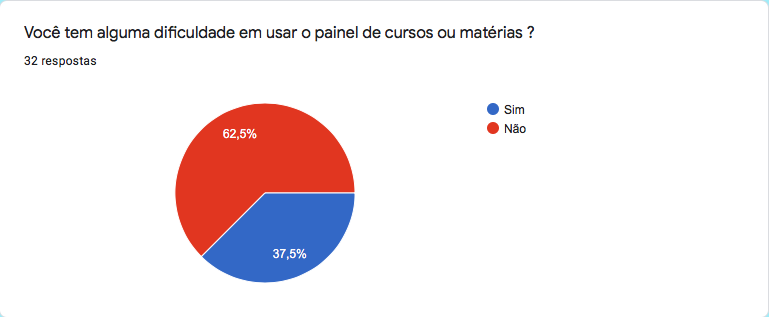
\includegraphics[width=.9\linewidth]{./media/grafico_painel.png}
\caption{\label{fig:orgab6de9a}Porcentagem de alunos que consideram ter dificuldade de usar o painel de cursos da plataforma.}
\end{figure}
\end{document}
